% % % % % % % % % % % % % % % % % % % % % % % % % % % % % % % % % % % % % % % % % % % %
%                                                                                     %
% Short Sectioned Assignment LaTeX Template Version 1.0 (5/5/12)                      %
% This template has been downloaded from: http://www.LaTeXTemplates.com               %
%                                                                                     %
% Original author:  Frits Wenneker (http://www.howtotex.com)                          %
%                                                                                     %
% Modified by: Fco Javier Sueza Rodríguez (fcosueza@disroot.org)                      %
%                                                                                     %
% Changes:                                                                            %
%           - Document type scrarticle                                                %
%           - Use babel-lang-spanish package and marvosym                             %
%           - Use hyperref, enumitem and tcolorbox                                    %
%           - Use fancyhdr package an configure it                                    %
%           - Use Time New Roman (mathptmx), Helvetic and Courier fonts               %
%                                                                                     %
% License: CC BY-NC-SA 3.0 (http://creativecommons.org/licenses/by-nc-sa/3.0/)        %
%                                                                                     %
% % % % % % % % % % % % % % % % % % % % % % % % % % % % % % % % % % % % % % % % % % % %

%-----------------------------------------------%
%	              Packages                  %
%-----------------------------------------------%

\documentclass[bibliography=totoc]{scrarticle}

% ---- Text Input/Output ----- %

\usepackage[T1]{fontenc}
\usepackage[utf8]{inputenc}
\usepackage{mathptmx}
\usepackage[scaled=.92]{helvet}
\usepackage{courier}
\usepackage[indent=12pt]{parskip}
\usepackage[titletoc, title]{appendix}

\usepackage{geometry}
\geometry{verbose,tmargin=3cm,bmargin=3cm,lmargin=2.5cm,rmargin=2.5cm}

% ---- Language ----- %

\usepackage[spanish, es-tabla, es-noquoting]{babel}
\usepackage{marvosym}

% ---- Another packages ---- %

\usepackage[toc, sort=use]{glossaries}
\usepackage{amsmath,amsfonts,amsthm}
\usepackage{graphics,graphicx}
\usepackage{tcolorbox}
\usepackage{hyperref}
\usepackage{enumitem}
\usepackage{fancyhdr}
\usepackage{float}
\usepackage{ulem}


%--------------------------------------------------------------------%
%                      Customizing Document                          %
%--------------------------------------------------------------------%

% -------------- Customize headers and footers---------------------- %

\pagestyle{fancy}

\fancyhead[]{}
\fancyfoot[L]{}
\fancyfoot[C]{}
\fancyfoot[R]{\thepage}

\renewcommand{\headrulewidth}{0pt} % Remove header underlines
\renewcommand{\footrulewidth}{0pt} % Remove footer underlines

% Needed to get first page footer correctly
\fancypagestyle{plain}{
    \fancyhf{}
    \fancyfoot[R]{\thepage}
}

% --------------------- Packages Configuration --------------------- %


\hypersetup{
    colorlinks=true,
    linkcolor=magenta,
    urlcolor=magenta
}

\setcounter{secnumdepth}{4}
\setcounter{tocdepth}{4}
\graphicspath{{./images/}}

\setlength{\headheight}{13.6pt} % Customize the height of the header
\numberwithin{figure}{section} % Number figures within sections
\numberwithin{table}{section}

% ------------------------ New Commands ----------------------------- %

\newcommand{\horrule}[1]{\rule{\linewidth}{#1}} % Create horizontal rule command

% ------------------------ Anexx now with name in spanish before title ----------------------- %

\addto\captionsspanish{%
	\renewcommand\appendixname{Anexo}
	\renewcommand\appendixpagename{Anexos}
}




%----------------------------------------------------------------------------------------
%	TÍTULO Y DATOS DEL ALUMNO
%----------------------------------------------------------------------------------------

\title{
\vspace{10ex}
\normalfont \normalsize
\huge \textbf{Sistemas de Big data}
}
\author{Francisco Javier Sueza Rodríguez}
\date{\normalsize\today}

\glsenablehyper
\makeglossaries
\loadglsentries{glos}

%----------------------------------------------------------------------------------------
%                                     DOCUMENTO
%----------------------------------------------------------------------------------------
\begin{document}


\maketitle

\thispagestyle{empty}

\vspace{75ex}

\begin{center}
    \begin{tabular}{l l}
        \textbf{Centro}: & IES Zaidin-Vergeles \\
        \textbf{Curso}: & Inteligencia Artificial y Big Data\\
        \textbf{Asignatura}: & Sistemas de Big Data\
    \end{tabular}
\end{center}

\newpage

\begingroup
\hypersetup{linkcolor=black}
\tableofcontents
\endgroup

\newpage

\begingroup
\hypersetup{linkcolor=black}
\listoffigures
\listoftables
\endgroup

\newpage

\section{Introducción a Big Data}
En esta primera unidad vamos a realizar una \textbf{introducción al Big Data}. Comenzaremos entendiendo cuales han sido las circunstancias del surgimiento del Big Data. Veremos también que son los clústeres de computadoras, que forma la infraestructura básica de los sistemas de Big Data. 

Además, veremos conceptos muy importantes para entender el fenómeno del Big Data. Finalmente ver la arquitectura en capas que se utiliza en en proyecto de Big Data hoy en día.

\subsection{Por qué Big Data}
En una empresa o institución, la \textbf{cantidad de datos} que se generan pueden llegar a ser enormes. Si la cantidad de datos es muy enorme, los \textbf{métodos tradicionales} pueden \textbf{no ser suficientes} para gestionar, de forma eficiente estos datos. Aquí es donde entra en juego el \textbf{Big Data}, un conjunto de tecnologías y metodologías que permiten gestionar grandes cantidades de datos de forma más eficiente, y en esta sección vamos a ver las características que lo hacen necesario.

\subsubsection{Las 5 Vs}
En esta sección vamos a ver las \textbf{cinco características} de Big Data que suelen usarse para discernir si el procesamiento de datos que necesitamos realizar puede realmente considerarse como Big Data.

Esas 5 características se llaman "\textbf{las 5 Vs}" y se componete de: \textbf{volumen}, \textbf{velocidad}, \textbf{variedad}, \textbf{veracidad} y \textbf{valor}. A continuación, vamos a describir con más detalle estas características.

\paragraph{Volumen}
~\\\\
\-\ \-\ \-\ La primera característica de reto del Big Data es el \textbf{gran volumen de datos} que hay que procesar, es decir, la cantidad de bytes de información que hay que tratar.

En los últimos tiempos, la \textbf{cantidad de información} que hay que procesar ha ido creciendo de forma exponencial, ya todo esta digitalizado, los usuarios interactúan de forma online con las administraciones, las empresa tiene que almacenar datos de sus clientes o usuarios, ...etc. Para que nos hagamos la idea de la magnitud de esta cantidad de datos, podemos ver una tabla en la Figura 1.1 donde se muestran todas las magnitudes que miden la cantidad de información.

Hay que tener en cuenta que si bien el significado de un kilobyte (KB) es de 1000 bytes, dado que en ambientes computacionales se emplea constantemente la numeración en base 2, existe el \textbf{kibibyt} (KiB), el cual corresponde a 1024 bytes (\(\ 2^{10} \)). De igual modo también existe el \textbf{mebibyte}  (MiB = \(\ 2^{20} \)), \textbf{gibibyte}  (GiB = \(\ 2^{30} \)), y así toda la progresión hasta llegar al \textbf{yobibyte} (YiB = \(\ 2^{80} \)).

Lo que puede producir cierta confusión es que por lo general se suele usar la nomenclatura en base 10 de forma indistinta, para referirse tanto a la base 10 como la base 2. Es decir, cuando vemos 1 MB, ses posible que signifique $10^{6}$ bytes, pero también es posible que signifique $2^{20}$ bytes. Puede depender tanto del fabricante del dispositivo, como que nos estemos refiriendo, como RAM, hardware de red, ...etc.

Para hacernos una idea del volumen de datos que maneja la humanidad, según el volumen de \textbf{datos en el mundo} se calculaba en unos \textbf{4.4 zettabytes en 2013}, teniendo para el \textbf{año 2025 163 zettabytes}.

\begin{figure}[ht]
	\centering
	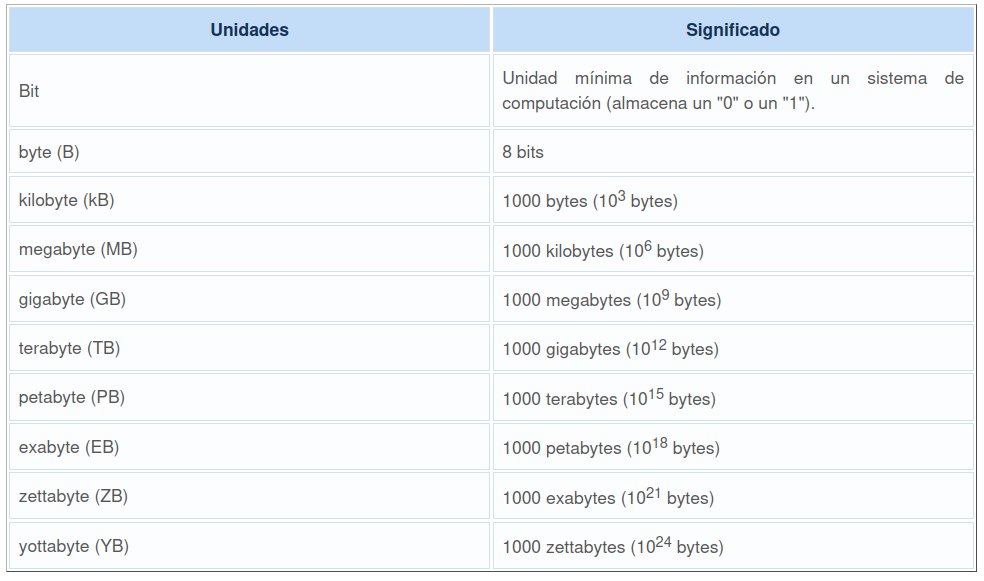
\includegraphics[scale=0.60]{magnitud-bit.png}
	\caption{Unidades de cantidad de información}
\end{figure}

Hay que tener en cuenta que \textbf{no hay una cantidad fija} a partir de la cual se pueda considerar que el problema es Big Data. Simplemente nos quedaremos con que los sistemas de Big Data manejan del orden de \textbf{petabytes} (PB) o \textbf{exabytes} (EB). Pero y, ¿de dónde vienen todos estos datos? Algunas de las \textbf{principales fuentes} de estos datos son:

\begin{itemize}
	\item Datos de \textbf{usuarios y/o clientes} de instituciones y empresas.
	\item Datos generados por \textbf{transacciones} (compras, transferencias,...)
	\item Datos adquiridos por \textbf{sensores} (temperatura, humedad, ...)
	\item Datos subidos a \textbf{redes sociales} (fotos, textos, ...)
	\item Datos relacionados con la salud (historiales, resultados, ...)
	\item Datos de geolocalización (GPS)
	\item Datos guardados en logs (accesos a web, de aplicaciones, ...)
	\item Datos producidos por le internet de las cosas (dispositivos IoT)
	\item Datos producidos por las ciencias (experimentos, genómica, meteorología, ...)
	\item Datos producidos por cámaras (imágenes, videos, ...)
	\item Datos Open Data (datos liberados o abiertos por instituciones)
\end{itemize}

Mención especial requieren los \textbf{datos abiertos}, ya que son una fuente interesante de datos. Podemos consultar más información en su \href{https://es.wikipedia.org/wiki/Datos_abiertos}{entrada de Wikipedia}. En concreto, en España, podemos encontrar la \href{https://datos.gob.es/es/}{web del gobierno del España} relativa a este proyecto, donde podemos encontrar todos los datos liberalizados por el gobierno los diferentes gobiernos de España.

\paragraph{Velocidad}
~\\\\
\-\ \-\ \-\ No solo es relevante la cantidad de datos con los que tratamos, sino que también es importante la \textbf{velocidad a la que se producen}. Para hacernos una idea, se calcula que en el \textbf{mundo se general} cada \textbf{60 segundos}: 

\begin{itemize}
	\item 350.000 tweets
	\item 300 horas de video subido a YouTube
	\item 171 millones de correos electrónicos
	\item 330 GBs de información generados por sensores
\end{itemize}

Si volvemos a revisar la lista de fuentes de datos del punto anterior y tenemos en cuenta que en el mundo hay 7870 millones de personas (datos de 2022), podemos hacernos una idea de la velocidad a la que se generan los datos cada minuto que pasa. Y el problema no es solo a la velocidad a la que se generan los datos, sino que hay que procesarlos e integrarlos a igual velocidad.

A raíz de esto, se han creado nuevas estrategias como el \textbf{procesamiento tipe streaming}, del que hablaremos más adelante.                                              

\paragraph{Variedad}
~\\\\
\-\ \-\ \-\ Además, de la cantidad de datos y la velocidad a la que se generan, existe el problema de la \textbf{variedad de datos} que se generan, en lo relativo a su representación. Dentro de esta variedad, podemos encontrar los siguientes grupos:

\begin{itemize}
	\item \textbf{Datos Estructurados}
	
	Los datos estructurados son aquellos que \textbf{existen en bases de datos}, los cuales existen dentro de tablas con una estructura bien definida que nos indica que tipo de datos es cada una de las columnas.
	
	\item \textbf{Datos No Estructurados}
	
	Son aquellos que no  se rigen por un esquema, como pueden ser \textbf{vídeos}, \textbf{imágenes} o \textbf{audios.}
	
	Hay que tener en cuenta que la proporción de datos no estructurados del mundo se estima que sean sobre un 80\% de los datos totales, lo cual se debe a la naturaleza de éstos datos. Solo hay que comprar el espacio de almacenamiento que ocupa un vídeo o una canción en comparación con el que ocupa un registro en una base de datos.
	
	\item \textbf{Datos Semiestructurados}
	
	Son datos definidos con una cierta estructura pero que no tienen una naturaleza relacional, como en una base de datos. Por lo general se almacenan en ficheros de texto siguiendo un formato preestablecido, de modo que mantienen la flexibilidad que ofrece el fichero, a la vez que es posible determinar que significa cada una de las porciones de información que se encuentran en el mismo.
	
	Algunos ejemplos de este tipo de ficheros son: \textbf{CSV}, \textbf{XML} y \textbf{JSON}.
	
	\item \textbf{Metadatos}
	
	Los metadatos son datos extra, que se generan de forma automática a veces, y que contienen \textbf{información sobre los propios datos}. Algunos ejemplos de la información que se pueden almacenar son los siguientes:
	
	\begin{itemize}
		\item Información sobre la estructura del dato.
		\item Fuente.
		\item Autor.
		\item Fecha de creación.
		\item Resolución en pixeles (imágenes o vídeos).
		\item Duración (vídeos).
		\item Tasa de muestreo (audio).
		\item Tipo de compresión.
	\end{itemize}
	
	Estos son algunos, aunque los metadatos pueden almacenar cualquier tipo de información que nos pueda ayudar a interpretar los datos que se han almacenado.
\end{itemize}

\paragraph{Veracidad}
~\\\\
\-\ \-\ \-\ Un problema extra con el que hay que tratar es que los datos no siempre cuentan con la calidad deseada o no son \textbf{totalmente fieles a la realidad}. 

Este concepto esta íntimamente ligado con el concepto de \textbf{señal/ruido} en el flujo de información. El \textbf{ruido} son datos que no pueden ser convertidos en información, mientras que la \textbf{señal} esta constituida por los datos que sí se pueden convertir en información. 

Así, por un lado, es necesario conocer en que condiciones se adquirieron los datos, para poder estimar su veracidad, mientras que en otras situaciones será necesario realizar un procesamiento específico de los mismos con el fin de resolver posibles problemas o eliminar información no válida (ruido).

Por norma general, los datos generados de forma automática contienen menos ruido que los que producen las personas.

\paragraph{Valor}
~\\\\
\-\ \-\ \-\ La última de las 5 Vs es el \textbf{valor}, concepto ligado a cómo de útiles son los datos para una institución, empresa o persona, y que esta íntimamente ligado con el concepto de \textbf{veracidad}, ya que cuanto más veraces sean los datos más valor se puede obtener de ellos. 

También depende en gran medido del \textbf{tiempo transcurrido} desde que se produjeron esos datos. Por ejemplo, si estamos operando en bolsa, los datos sobre el valor de las acciones tiene mucho valor si se han generado hace 1 segundo que si se lo han hecho hace 10 minutos. En este aspecto, cuanto más rápido se hagan llegar los datos desde donde se producen hasta donde se toman las decisiones, mas valor tendrán.

Es importante, además, que los datos sean \textbf{lo más completos posible} para poder producir el valor deseado. Es decir, además de ser veraces deberán estar completos, incluyendo todo lo que se necesita para interpretar correctamente lo que representan.

Por último, la \textbf{propia interpretación del dato} también juega un papel vital. Sería absurdo, por ejemplo, tener almacenadas las temperaturas de un sensor que esta debajo de tierra e intentar usar esos datos para predecir la temperatura ambiente. En este caso, aunque el dato es veraz y completo, la interpretación estaría siendo errónea.

\subsubsection{Que Conseguimos Gracias al Big Data}
En esta sección vamos a ver que nos aporta, no solo obtener y almacenar grandes cantidad de datos, sino también poder tratarlos y analizarlos gracias a las tecnologías de Big Data.

Las \textbf{metodologías para Big Data} nos permiten realizar diversas operaciones con grandes cantidades de datos, entre las cuales se encuentra:

\begin{itemize}
	\item Capturarlos desde sus orígenes.
	\item Integrarlos para poder almacenarlos de forma unificada.
	\item Almacenarlos de un modo distribuido y replicado, consiguiendo alta disponibilidad.
	\item Tratarlos de forma distribuida usando un gran numero de máquinas que los procesan en paralelo.
	\item Aplicar técnicas de minería de datos para crear modelos predictivos.
	\item Usar esos modelos para realizar predicciones a utilizar en sistemas automáticos.
	\item Crear visualizaciones y cuadros de mando usando tanto los propios datos como los modelos creados con ellos.
\end{itemize}
\newpage
 
\printglossary	

\newpage

\bibliography{citas}
\bibliographystyle{unsrt}


\end{document} 